\documentclass[12pt]{article}
\usepackage[left=1in, right=1in, top=1in, bottom=1in]{geometry}
\usepackage{graphicx}
\usepackage{url}
\usepackage{cite}
\usepackage{float}
\usepackage{caption}
\usepackage{subcaption}
\usepackage{hyperref}
\hypersetup{
    colorlinks,
    citecolor=black,
    filecolor=black,
    linkcolor=black,
    urlcolor=black
}

\renewcommand{\familydefault}{\sfdefault}


\begin{document}
\begin{titlepage}
    \begin{center}
        \LARGE
        \textbf{ELE 401 - GRADUATION PROJECT I}

        \Large
        \textbf{SECOND INTERIM REPORT}

        \vspace{70pt}

        \textit{
            Hacettepe University \\
            Department of Electrical and Electronics Engineering
        }
    \end{center}

    \vspace{90pt}

    \large

    \textbf{Project Title:} Sensor Fusion in the Cloud \\

    \textbf{Project Group Members:} Ertuğrul Tiyek, Ahmet Yusuf Şirin

    \vspace{30pt}

    \textbf{Project Supervisor:} Asst. Prof. Dr. İsmail Uyanık \\

    \textbf{Submission Date:} 11.12.2022

    \vspace{\fill}

    \begin{center}
        \textit{FALL 2022-2023}
    \end{center}
\end{titlepage}

\clearpage

\tableofcontents
\listoffigures
\listoftables

\clearpage

\begin{abstract}
    From the point on we are studying on the sensor fusion. In this report we will briefly emphasize the legged robot usage for our final decisions. On the other hand, the concept ot the sensor fusion and the alternative methodologies to implement it correctly to serve the main purpose of sensor fusion, that is reliable odometry data extraction.
\end{abstract}

\section{INTRODUCTION}

One of the most important aim of the modern technology is the sensing the environment. Living beings have sense organs to know the environment. They have brains to make fusion the sensor data and augment the environmental information taken from sense organs. For example, human standing in balance, we can say that they use the data coming from their eyes and ears together.

People are studying to make this sensing and augmenting artificially, too. They use computers to achieve this. But computers cannot sense the environment directly. They need some devices called sensors. There are all kinds of sensors to measure different environmental quantities. For same quantity, there are different sensors using different technologies, have different precision and accuracy levels. Each sensor has its advantages and disadvantages. Even sensors that are serving a different purpose can help to augment same information other than their main. This is known as "sensor fusion"~\cite{enwiki:1115352853}. Just like humans, robots are use camera and inertial sensors to stand in balance.

In our project, sensor fusion handles extracting depth information. Sensor fusion can be implemented using specific algorithms like EKF, CNN etc. according to quantity that will be calculated, number and types of sensors used, accuracy and performance needed. We are planning to develop a sensor fusion algorithm with the help of living organisms. As we mentioned before, living beings perform sensor fusion perfectly. We will be examining the zebra fish and how it processes data of its sense organs to produce depth information. Then we will try to develop similar algorithm or improve our algorithm with data taken from zebra fish.

Depth information can be used for many applications like automatic driven vehicles, UAVs, Augmented Reality devices and 3D modeling of areas. Our concept in this project will be autonomous controlled SLAM Robot. Simultaneous localization and mapping (SLAM) is the computational problem of constructing or updating a map of an unknown environment while simultaneously keeping track of an agent's location within it~\cite{enwiki:1120084976}. We use a robot to move the system.

Another concept we aim to use is cloud computing. Mobile computing devices may not match the performance requirements in some cases. To achieve more accurate depth information, complex control algorithms or neural networks will be used in our project which needs high computing power. As an alternative to the mobile computing devices, we may use cloud computing.


\section{METHODS}

The definition of our project is explained in detail in the first interim report. In the light of the definition, we try to make the decisions and the design parameters clear. To sake of easiness we draw some paths going same destination and arguing to reach the optimal path on the alternatives. Those alternatives are listed and described below. Then we will clearly elucidate our method now.

Since the project includes plenty of areas to work those are distinct, we divide them into subtopics. Those are:

\begin{enumerate}
    \item Sensor Choosing Methods
    \item Sensor Fusion Methods
    \item Sensor Data Enhancement Methods
    \item Fusion Data Enhancement Methods
\end{enumerate}

\subsection{Sensor Choosing Methods}

Our aim in this project is to achieve high reliability by using (fusing) all the sensors we have together. However, when we want to do all these together, we foresee that the project will reach very different dimensions. Therefore, while continuing the project, we decided to select a number of sensors in order to focus on algorithm development.

We set ourselves criteria when choosing sensors. Easy to use sensors is one of our main priorities due to our job description. In addition, considering the algorithmic complexity, working with sensors with linear system response is also an important criterion. In addition, the frequency of receiving data from the sensor is of great importance. Because if the sensor data we will fuse does not come at the same frequency, we will need to add operations to our algorithm to make the sensor frequencies equal by upsampling and downsampling.

We basically divided the sensors we have into two groups as those producing RGBD data or those producing Depth Point Cloud data.

\subsubsection{Method 1: Internal Sensor Using}
The internal sensors of the legged robot include five pairs of stereo cameras that produce RGBD data, and ultrasonic sensors that produce Depth Point Cloud data when viewed cumulatively, SuperSensorySystem. In addition to these, each foot has pressure sensors and an internal IMU.

\subsubsection{Method 2: External Sensor Using}
Our external sensors are ZED Stereo camera which produces RGBD data, Velodyne 3D LiDAR which produces Depth Point Cloud data and Xbox 360 Kinect having 3D depth sensor, RGB camera, microphone array, and also tilt motor. In the future, it is also possible to add sensors such as IMU and GPS to support odometry information.

\subsubsection{Method 3: Mixed Sensor Using}
We can also use our sensors mixed. However, complexity will increase in this method and the workload to be done before the sensor fusion algorithm will become more.


\begin{itemize}
    \item \textbf{Internal Unitree Camera – Super Sensory System:} \\
          Lens Angle ~150°×170°

          \begin{figure}[H]
              \centering
              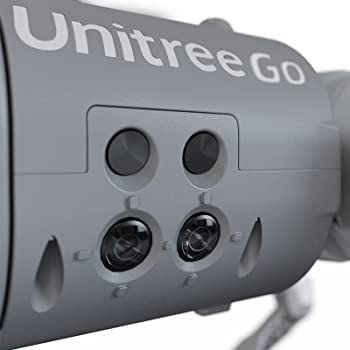
\includegraphics[width=0.5\textwidth]{SuperSensorySystem.png}
              \caption{Super Sensory System}
          \end{figure}

    \item \textbf{External ZED Stereo Camera:} \\

          \begin{figure}[H]
              \centering
              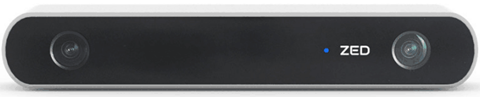
\includegraphics[width=0.5\textwidth]{ZEDCam.png}
              \caption{ZED Stereo Camera~\cite{ZEDStereoCamera}}
          \end{figure}

          Some specifications of ZED:

          \begin{itemize}
              \item High-Resolution and High Frame-rate 3D Video Capture (1080p 30fps)
              \item Depth Perception indoors and outdoors at up to 20m
              \item 6-DoF Positional Tracking
              \item Spatial Mapping
              \item 110° Wide Angle Cameras
          \end{itemize}

    \item \textbf{Xbox 360 Kinect:} \\
          \begin{figure}[H]
              \centering
              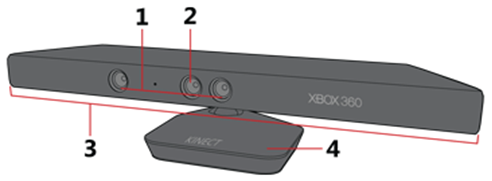
\includegraphics[width=0.5\textwidth]{XBoxKinect.png}
              \caption{Xbox 360 Kinect~\cite{XboxKinect}}
          \end{figure}

          \begin{enumerate}
              \item 3D Depth sensor (IR Emitter + IR Camera / Depth Sensor)
              \item RGB camera (Color Sensor)
              \item Microphone array
              \item Tilt motor (for detecting floor and players in the play space)
          \end{enumerate}

    \item \textbf{Velodyne 80-VLP-16-A 3D LiDAR:} \\
          \begin{figure}[H]
              \centering
              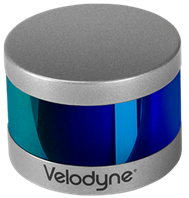
\includegraphics[width=0.3\textwidth]{LiDAR.png}
              \caption{Velodyne LiDAR}
          \end{figure}

          Some specifications of LiDAR:

          \begin{itemize}
              \item 100 m Range
              \item 360° x 30° Viewing Angle
              \item 0.3 Million Points/Second
              \item 100Mbps Ethernet \& UDP Interface
              \item Rated IP67
          \end{itemize}
\end{itemize}

We have taken all these into consideration while doing the preliminary design, and together with the evaluations under the following headings, we have determined a starting point for ourselves. You can find the details under the Preliminary design heading.

% Stereo Camera Decision Method
% LiDAR Decision Method
% Internal IMU usage on legged robot
% Documentation about sensors in marketplace and we owned (engineering decisions on costs)


\subsection{Sensor Fusion Methods}

\subsubsection{Method 1: Complementary Filter}
We wanted to set out using known methods for sensor fusion. In this way, we aimed to improve the performance we want to achieve with methods that we understand fundamentally, instead of using the resources in the literature directly. In fact, we started out by examining the usages of Kalman filter and extended Kalman filter, which are quite commonly used for state estimations made from aircraft IMU sensors, in this field. We predicted that if you continue on your way by choosing the most primitive complementary filter among them, we will be able to understand more clearly that we are moving away from the target in every development we make.

\begin{figure}[H]
    \centering
    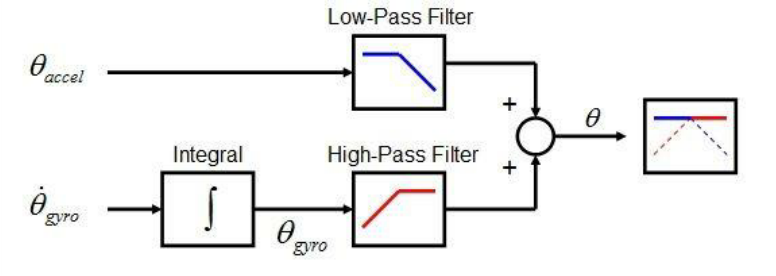
\includegraphics[width=0.7\textwidth]{CF.png}
    \caption{Complementary Filter Example for Aircraft Attitude}
\end{figure}

\subsubsection{Method 2: Kalman Filter}
Using the Kalman filter is also a method between using the extended Kalman filter and using a complementary filter. Since we want to use it with some methods that will enhance compelemntery filtery, we have already produced our own gain function. However, we also considered the Kalman filter as a method.

\begin{figure}[H]
    \centering
    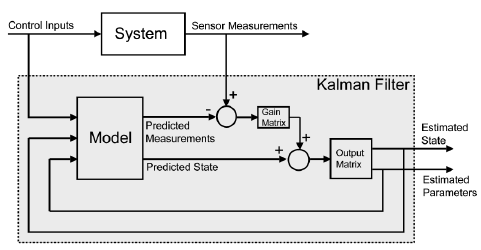
\includegraphics[width=0.7\textwidth]{KF.png}
    \caption{Kalman Filter Example for Aircraft Attitude}
\end{figure}

\subsubsection{Method 3: Extended Kalman Filter Method}
In addition to previous methods, we also evaluated the opinion that preliminary design can speed up the process by directly using the most advanced extenden Kalman filter. However, unlike in the aircraft scenario, we could not find an example use for depth data to be suitable for our scenario~\cite{9307398}.

\begin{figure}[H]
    \centering
    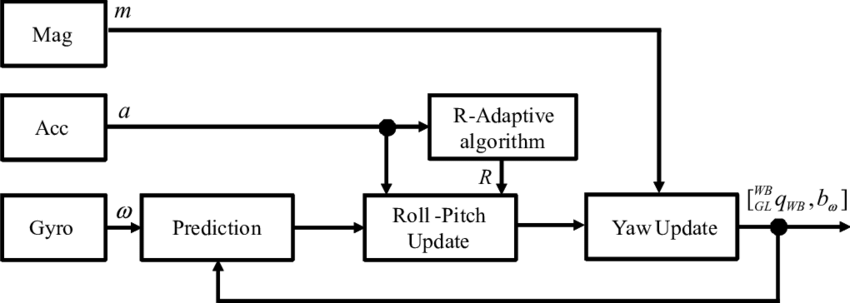
\includegraphics[width=0.7\textwidth]{EKF.png}
    \caption{Extended Kalman Filter Example for Aircraft Attitude}
\end{figure}

A comparison in which the models in which the state estimator methods are effective and the noise characteristics are given together is given in the X table, cost function comparisons for further analysis~\cite{The_cost_function_of_the_data_fusion_process_and_i}.

\begin{table}[H]
    \centering
    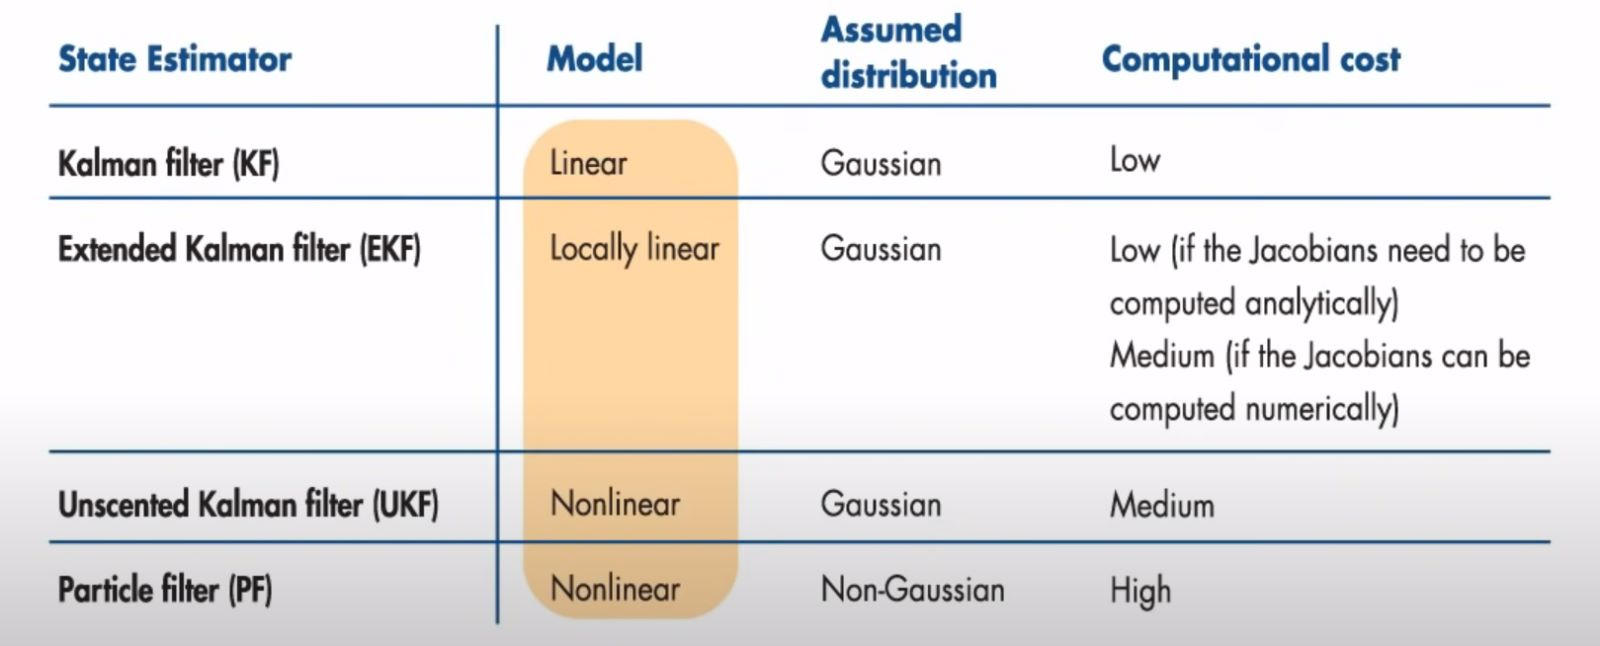
\includegraphics[width=0.8\textwidth]{CostComparison.jpeg}
    \caption{Cost Function Comparison}
\end{table}


\subsection{Sensor Data Enhancement Methods}

We compare the following methods for data enhancement to following data fusion.

\subsubsection{Method 1: Only Data Rate and Range Matching}
Since the data we want to obtain is odometry, we evaluated creating parametric inputs in the methods we used while continuing the project. Because we sould think about Sensor Data Rate - State Estimation Relation. In this way, we aimed to analyze whether we could establish a relationship between the quality of the raw data and the esimated odometry data. After some tests we will briefly report our results about early sensor data enhancement for sensor fusion.

\subsubsection{Metod 2: Papoulis-Gerchberg Algorithm for Depth Point Cloud}
We are searching about Papoulis-Gerchberg algorithm effects on LiDAR and Stereo depth map results to enhance the data resolution before data fusion. An image super-resolution method, the Papoulis–Gerchberg (P–G) algorithm, on range data represented in the form of a greyscale image. However, the low convergence rate of the original P–G algorithm impedes its use for online applications~\cite{ozbay2015high, kuzucu2018enhancing}. By referencing this method we also proposed as an enhancement method.~\cite{6280128}


\section{PRELIMINARY DESIGN}

ZED stereo camera and Velodyne 3D LiDAR were chosen for the preliminary design, which are sensors that are well-documented, have a large community, and are easier to use and access resources than the internal sensors of the legged robot. This sensor will also minimize the complexity of the algorithm to be used in sensor fusion, as they offer a wide resolution and data rate band.

As the sensor fusion algorithm, it was ordered from simple to complex or from low to high performance, and it was decided to make a start with a complementary filter. Again, it was decided to use methods such as edge preservation~\cite{9307398} as an aid to the main algorithm in order to increase the sensor fusion performance.

We choose the complementary filter for fusing the depth information of two sensors. Each sensor has its own properties, advantages and disadvantages. According to these characteristics of sensors we tune our sensor fusion algorithm. But like all control systems, we first regulate our input signals to work with.

Thing we have to match in these two sensors data is viewing angle. Stereo vision camera has a viewing angle upto 110°. We simply reduced the viewing angle of the 3D lidar to match the stereo vision cameras viewing angle. But further steps we are planning to use also 360° lidar information to enhance environmental data while performing SLAM.

Raw data provided by lidar and stereo vision cameras in different formats. Stereo vision camera extracts depth frames as well as RGBD (Red Green Blue Depth) in cartesian form. 3D lidar extracts data in point cloud form which is basically in spherical form. In the other hand the resolution of stereo vision data is available in 2208x1242 at 15 fps, 1920x1080 at 30fps, 1280x720 at 60 fps, 672x376 at 100 fps. The 3D lidar works completely different and samples much less data. In order to match the sampled data from two sensors, we decided upsampling the lidar data and converting it to cartesian form. We use dynamic Papoulis–Gerchberg algorithm to augment the lidar data and then linearly interpolate this information while converting point cloud data to depth frame.

Iterative Papoulis–Gerchberg algorithm is the method used to recover the lost samples of the signal. It is mostly used for super resolution images in image processing. In a single frame manner, iterative Papoulis–Gerchberg algorithm will be enough to increase data in a single point cloud of a lidar. But our aim is continuously matching the frames, we will use the dynamic Papoulis–Gerchberg algorithm. This algorithm make use of stillness of background and continuity of movement to reduce computational effort in Papoulis–Gerchberg.

There is also difference between sample rates of two sensors. Stereo camera samples frames in range of 15 to 100 frames per second. Lidar samples point clouds by rotating its lidar continuously. Each rotation provides one whole 360° sample (30° vertical). Lidar works in range 300 rpms to 600 rpms. That provides us 5-to-10 point clouds per second. We aim to up-sample the  number of point cloud per second by again linear interpolation.

There is one more problem with the lidar. Ability of lidar is not limited by the only rotation but also sample rate of sensor. Increasing rotation speed reduces the quality of the point clouds. One part of the project is experiencing the different data rates and calculating the processing effort, transmission capabilities and response times. So we will optimize resolution and data rates in the content of this project.

\subsection*{Sensor Fusion Algorithm}

We matched the formats of the input signals to keep the sensor fusion simple. There are two depth images as input signals to get more accurate depth image.

As a preliminary design, we are planning to calculate the depth image in per pixel fashion. As mentioned before, the complementary filter is formulated as:

\begin{equation}
    \hat{x} = \hat{x}_1 \alpha + \hat{x}_2 (1 - \alpha)
\end{equation}

We will generate $\alpha$ generation function to calculate $\alpha$ for each pixel and condition. Input sources are not functioning perfect in every conditions. There are some internal and external variables that effects the accuracy of measurement. Let’s observe these variables:


\subsubsection*{Variables That Effect Lidar:}

\begin{itemize}
    \item Beam Angle:

          3D lidar scans the environment in a three-dimensional manner. Velodyne VLP-16 scans 360° horizontally and 30° vertically. In different beam angles, Lidar accuracy depends. There is an article that contains more information about beam angle effect.

          \begin{figure}[H]
              \centering
              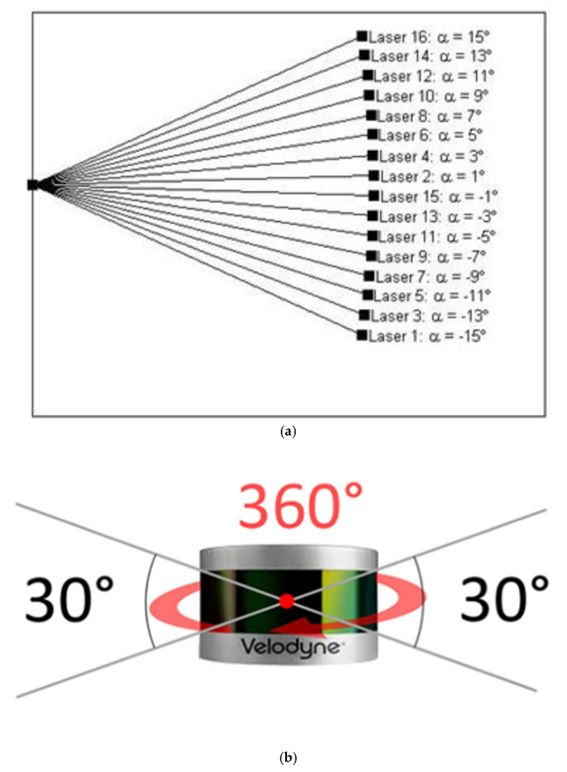
\includegraphics[width=0.5\textwidth]{LidarAngles.jpeg}
              \caption{Velodyne LiDAR Beam Angles~\cite{VelodynePerformance}}
          \end{figure}

    \item Rotation Speed:

          Sample rate of the lidar decreases as rotation speed of the lidar increases. It effects the quality of the depth image. But increasing the rotation speed provides us approximation to real time application.

    \item Distance:

          3D lidars can work in a range that is specified in datasheet. Out of this range, lidar cannot work properly. As we think of the working principle of the lidar, the processing time is not enough to measure too close points. The Velodyne VLP-16 model has a working range between 1m to 100m.

    \item Rough and Uneven Views:

          The Lidar is using wavelengths very close to visible light to observe visible objects. In some environments like forests, rough areas, rainy and foggy weathers there are lots of indentations like branches, twigs and leaves or water drops. Each of this bits and pieces prevents the infrared laser lights coming from lidar and creates canopies. Instead of a clean point cloud, lidar gets a noisy one.

          We can measure the effect of the bits and pieces in the environment to accuracy of lidar measurement by calculating the gradient of depth frame around target pixel.

          \begin{figure}[H]
              \centering
              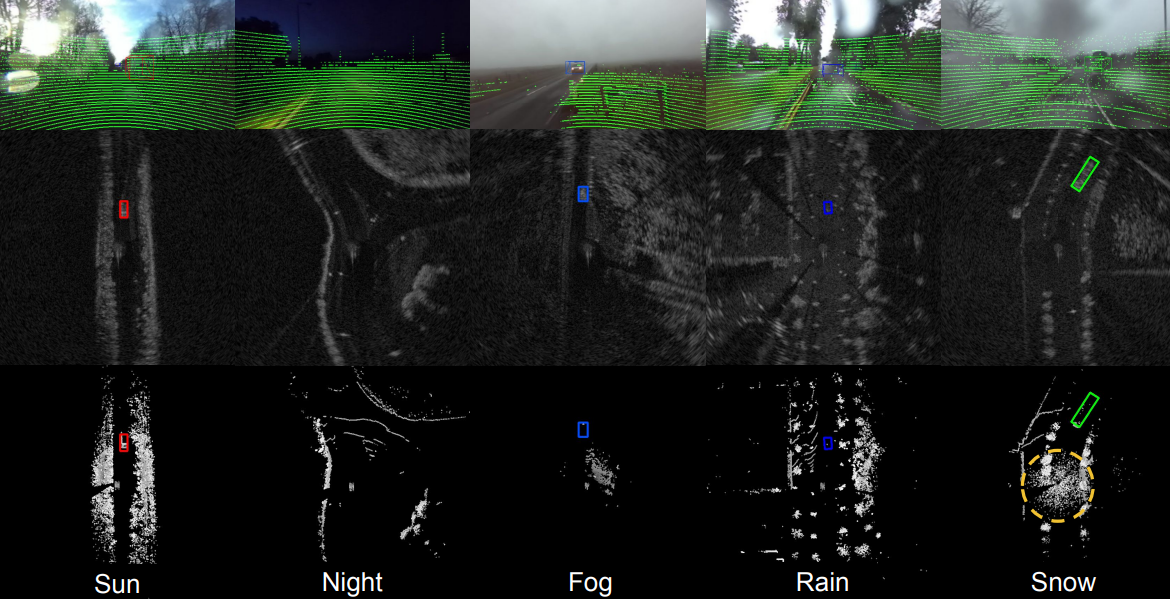
\includegraphics[width=0.9\textwidth]{LidarViews.png}
              \caption{Gradient of Depth Image Around Target Pixel Gives Roughness of the Environment~\cite{https://doi.org/10.48550/arxiv.2010.09076}}
          \end{figure}
\end{itemize}


\subsubsection*{Variables That Effect Stereo Vision Camera:}

\begin{itemize}
    \item Distance:

          According to viewing angles and algorithm used to extract depth information from stereo image, there is an uncertainty appears. And this uncertainty increases as distance of the pixel increases. Uncertainty reduces the confidence of the input as it increased.

          \begin{figure}[H]
              \centering
              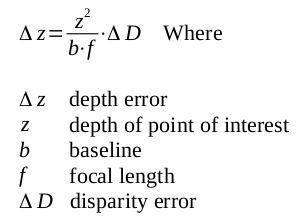
\includegraphics[width=0.4\textwidth]{CamDistance.png}
              \caption{Stereo Camera Depth Error Calculation~\cite{DisparityCalculator, gallup2008variable}}
          \end{figure}

    \item Brightness:

          The brightness of the environment is important for stereo vision depth estimation. As considering the working principles of the stereo vision depth estimation, there are two frames taken from different angles. First step is matching each pixel of left frame with corresponding pixel in right frame. This step includes computer vision algorithms like Sum of Squared Differences (SSD) and Sum of Absolute Differences (SAD). To perform matching properly, the frames should have well distributed histograms and good contrast values. If there is the brightness of frames are too high or too low, the algorithms cannot match the corresponding pixels.

          We can calculate the effect of brightness by observing the histogram of the RGB frames.
    \item Straight and no-Contrast Views:

          Like the brightness, the content of the frame is also important. If the frame includes low contrast, straight or similar patterns, the matching algorithms won’t work properly. For example, If the frame includes a flat white wall, the algorithm can not distinguish pixels in different frames. Likewise, if the frame has a periodic pattern like damas pattern, the algorithm also not work well.

          In this case we can calculate the effect of straightness by calculating gradient around target pixel in RGB frames.
\end{itemize}

According to these parameters, we will derive confidence generator functions that will calculate a confidence value for each input. By normalizing one of the confidence values will give us $\alpha$ value.

\begin{equation}
    \alpha = \frac{C_{LIDAR}}{C_{LIDAR} + C_{STEREO}}
\end{equation}

\begin{figure}[H]
    \centering
    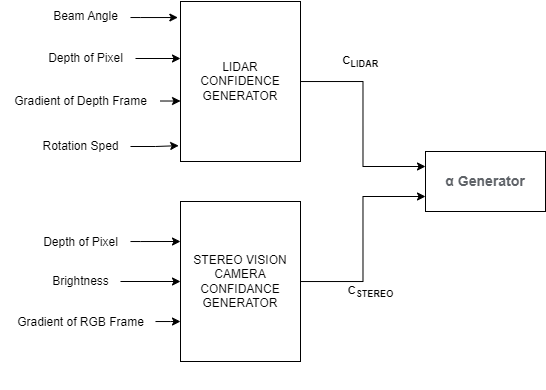
\includegraphics[width=0.9\textwidth]{AlphaFunction.jpeg}
    \caption{Alpha Function for Complementary Filter Enhancement}
\end{figure}

After extracting $\alpha$ value for each pixel of depth frame, we can simply apply complementary filter.

\begin{figure}[H]
    \centering
    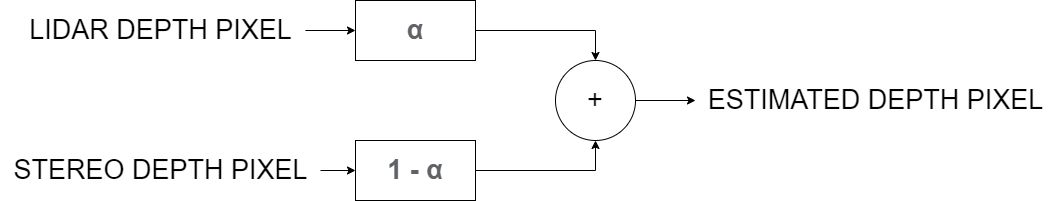
\includegraphics[width=0.9\textwidth]{CompFiltBD.jpeg}
    \caption{Complementary Filter Block Diagram}
\end{figure}

\addcontentsline{toc}{section}{REFERENCES}
\bibliographystyle{plain}
\bibliography{refs}
\end{document}